\Subsection{2.2 Знакомство с роботами TurtleBot, Maxwell и Pi Robot}




Для целей этой книги нам нужен робот, который мы можем, по крайней мере, запустить в симуляторе, чтобы проверить наш код. Репозиторий ros-by-example включает поддержку двух тестовых роботов, The \href{http://wiki.ros.org/action/show/Robots/TurtleBot?action=show&redirect=TurtleBot}{Willow Garage TurtleBot}, созданный \href{http://www.meloneewise.com/?page_id=31}{Melonee Wise }и \href{http://www.osrfoundation.org/team/tully-foote/}{Tully Foote} и собственный самодельный робот автора под названием \href{http://www.pirobot.org/}{Pi Robot}. 

Pi был вдохновлен \href{http://www.showusyoursensors.com/}{Michael Ferguson's Maxwell}, который, в свою очередь, был смоделирован по образцу робота \href{http://www.ros.org/news/2010/03/robots-using-ros-georgia-techs-assistive-robots.html}{El-E} компании Georgia Tech. Если у вас есть модель URDF вашего собственного робота, вы можете использовать его вместо одного из них. В любом случае, большая часть кода, который мы разрабатываем, будет работать практически на любом роботе, поддерживающем основные интерфейсы сообщений ROS.

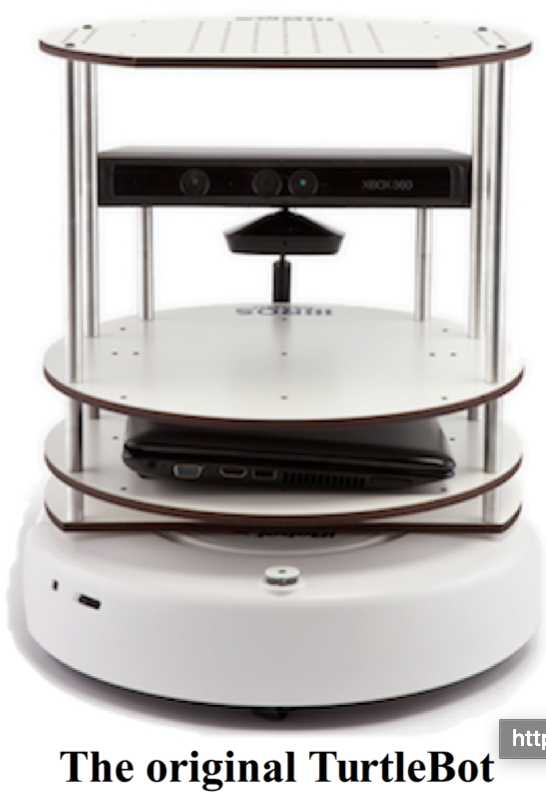
\includegraphics[width=9cm]{.gitbook/assets/snimok-ekrana-2020-05-29-v-21.27.59.png}

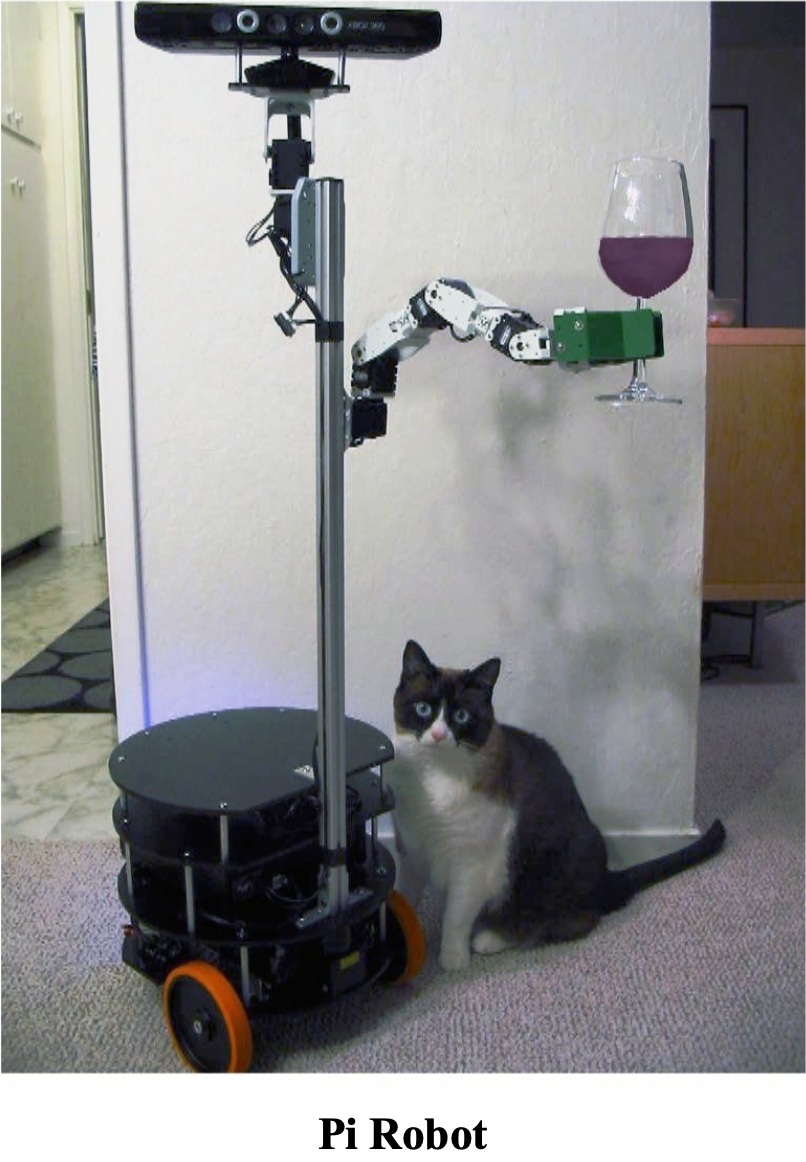
\includegraphics[width=9cm]{.gitbook/assets/snimok-ekrana-2020-05-29-v-21.29.59.png}

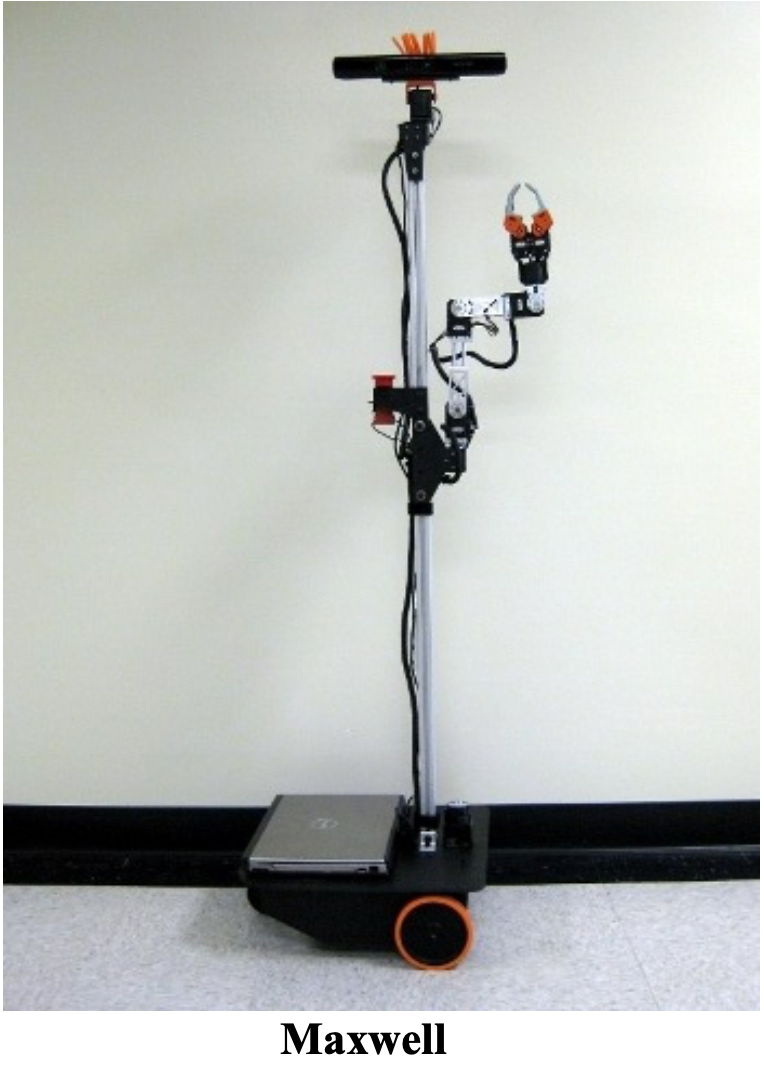
\includegraphics[width=9cm]{.gitbook/assets/snimok-ekrana-2020-05-29-v-21.29.44.png}

